 \begin{figure}
	\begin{center}
	%	\def\svgwidth{1.0\textwidth}
	%	\input{pics_tex/caustica1.pdf_tex}
	 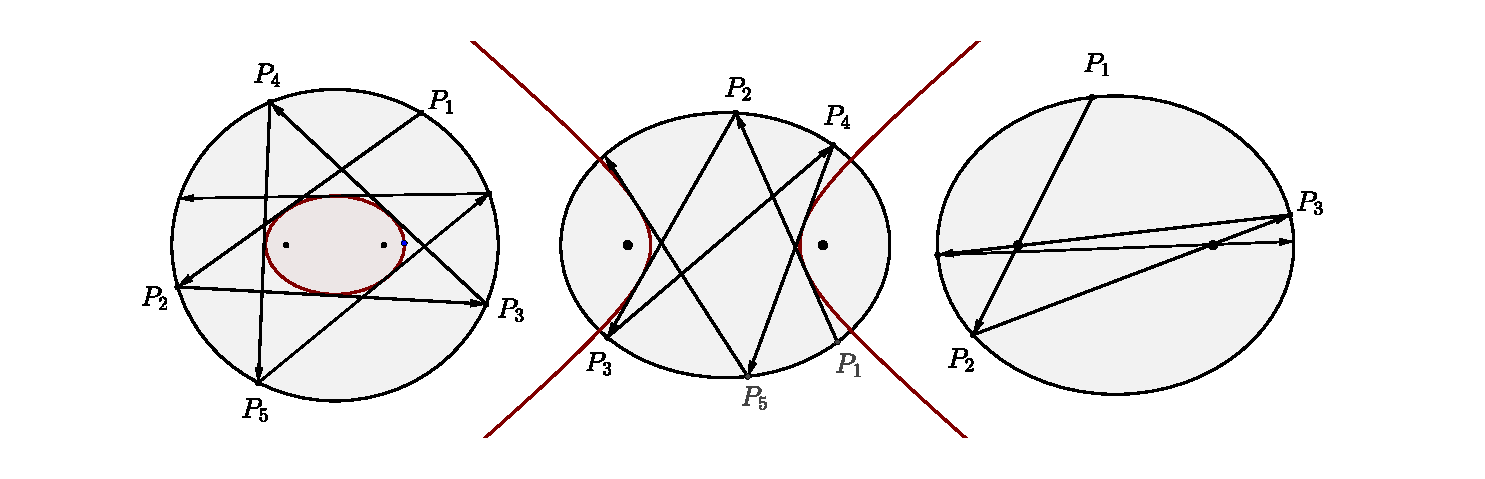
\includegraphics[scale=0.55]{chap_05/pics/pics-05-3tipos-orbitas.pdf}
		\caption{Three types of billiard orbits in the ellipse.}
	\end{center}
\label{fig:caustic1}
\end{figure} 
 
 \begin{theorem}
 Consider an  elliptic billiard defined  in the ellipse $\E$ given by $x^2/a^2+y^2/b^2=1$ $(a>b)$. Let $F_1=(-c,0)$ and $F_2=(c,0) $ the foci of $\E$. Let $(P_n)=(P_n)_{n\in\mathbb{Z}}$ be a billiard orbit inscribed in $\E$. Then:
 
 \begin{itemize} 
 \item[i)] If the segment of orbit $P_1 P_2$ is outside the segment $F_1F_2$ then the caustic of the orbit $(P_n)$ is a confocal ellipse $\E_c$ and the orbit is periodic or dense in the annulus defined by the pair  $\{\E,   \E_c \}$.
 
  \item[ii)] If the segment of orbit $P_1P_2$   intersects the segment $F_1F_2$ then the caustic of the orbit is a confocal hyperbola  $\Hc_1$ and the orbit is periodic or dense in the disk defined by the ellipse $\E$ and the caustic $\Hc_1$.
  
   \item[iii)] If the segment of orbit $P_1P_2$ pass through a focus  then the orbit pass through the other focus and is asymptotic to the 2-periodic orbit (diameter of the ellipse $\E$) in the past (backward) and  the future(forward).
\end{itemize}
\end{theorem}

 \begin{proof}
 We follow \cite{bry} to obtain the billiard map as a composition of two deck transformations.  Consider the pair of nested   ellipses parametrized by
 
 \begin{align*}
     \E:&\;\; f(z,w)=\frac{z^2}{a^2}+\frac{w^2}{b^2}-1=0\\
     \E_c:&\;\; g(x,y)= \frac{x^2}{a_c^2}+\frac{y^2}{b_c^2}-1=0.
 \end{align*}
 
 A tangent (oriented) line to $\E_c$ (caustic), passing through $q_0=(x,y)$ is given by
 \[h(x,y,z,w) =\frac{xz}{a_c^2}+\frac{yw}{b_c^2}-1=0.\]
 Now consider the set
 $\Sigma= \{(x,y,z,w): f(z,w)=g(x,y)=h(x,y,z,w)=0\}.$  
 The set $\Sigma$ is the union of two disjoint circles (curves  diffeomorphic  to circles) given by
 $\Sigma_+=\{p\in \Sigma: xw-yz>0\} $ and
  $\Sigma_-=\{p\in \Sigma: xw-yz<0\}. $
  Given $q_0\in\E_c$, let $p_0=(z,w)\in \E$ such that $(q_0,p_0)\in\Sigma_+.$ A line passing through $p_0$ and tangent to $\E_c$ passes through the point $q_1=(u,v)$ and $(u,v,z,w)\in\Sigma_-.$ 
 The projection  $\pi_1:\Sigma \to \E_c$ is a double cover. The same for the projection
 and $\pi:\Sigma\to \E$. 
 Now we observe that there is a unique map $\tau:\Sigma_{\pm}\to \Sigma_{\mp}$ such that $\tau(x,y,z,w)=(x,y,\bar{z},\bar{w})$. Here $(\bar{z},\bar{w})$ is the other point of intersection of the tangent line passing $(x,y)$ with the outer ellipse $\E$.
 
Also there is a unique map $\sigma:\Sigma_{\pm}\to \Sigma_{\mp}$ such that $\tau(x,y,z,w)=( \bar{x},\bar{y},z,w)$. The point $q_1=( \bar{x},\bar{y})\in\E_c$ is the in polar line of $p_0=(z,w)$. 
 
 %%%
 
 Therefore the billiard orbit can be defined as follows. For each $q_i\in \E_c$, let $p_i\in\E$ the point of intersection of tangent line at $q_i$ to $\E_c$ meets $\E$ with $(q_i,p_i)\in\Sigma_{+}$. Now let $q_{i+1}$ be the unique point on $\E_c$ such that $\{q_i,q_{i+1}\}$ are on the two tangent lines to $\E_c$ that pass through $p_i$. Therefore,   the map $q_i\to q_{i+1}$ is given by $\sigma\circ \tau$ (resp. $p_i\to p_{i+2}$) is an orientation preserving diffeomorphism on $\E_c$ (resp. on $\E$).

When the caustic is a hyperbola it is necessary to consider the second iteration to obtain an orientation diffeomorphism. See \cite{birkhoff1922} and \cite{kolod1985}.

Finally, when the orbit passes through a focus, the billiard map is conjugated with a diffeomorphism of the circle having two hyperbolic fixed points.
\end{proof}
 


\begin{figure}
	\begin{center}
	%	\def\svgwidth{1.0\textwidth}
	%	\input{pics_tex/bilharorbita.pdf_tex}
		 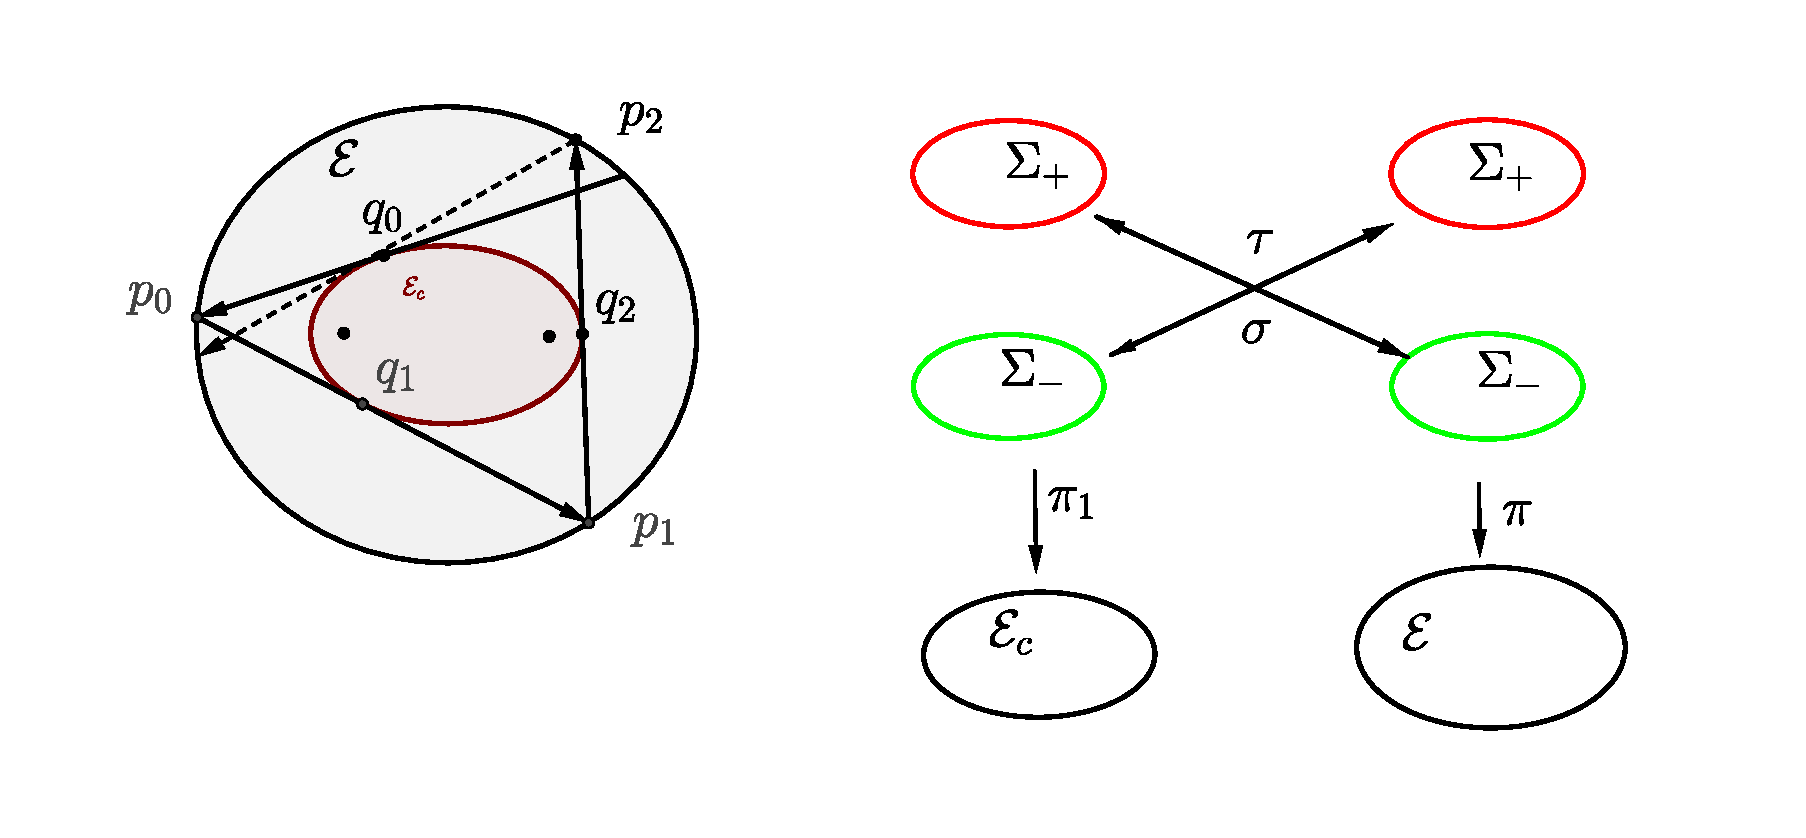
\includegraphics[scale=0.45]{chap_05/pics/pics-05-050-orbitas-dinamica.pdf}
		\caption{Maps $\sigma$, $\tau$ and the the diffeomorphism $\sigma\circ\tau$.}
	\end{center}
\label{fig:caustic2}
\end{figure}
